%
\documentclass{article}

% Recommended, but optional, packages for figures and better typesetting:
\usepackage{microtype}
\usepackage{graphicx}
\usepackage{subfigure}
\usepackage{booktabs} % for professional tables

% hyperref makes hyperlinks in the resulting PDF.
% If your build breaks (sometimes temporarily if a hyperlink spans a page)
% please comment out the following usepackage line and replace
% \usepackage{mlsys2023} with \usepackage[nohyperref]{mlsys2023} above.
\usepackage{hyperref}

% Attempt to make hyperref and algorithmic work together better:
\newcommand{\theHalgorithm}{\arabic{algorithm}}

% Use the following line for the initial blind version submitted for review:
\usepackage{mlsys2023}

% If accepted, instead use the following line for the camera-ready submission:
% \usepackage[accepted]{mlsys2023}

% The \mlsystitle you define below is probably too long as a header.
% Therefore, a short form for the running title is supplied here:
\mlsystitlerunning{Blockchain and Federated Learning}
\begin{document}

\twocolumn[
\mlsystitle{Blockchain and Federated Learning}

% It is OKAY to include author information, even for blind
% submissions: the style file will automatically remove it for you
% unless you've provided the [accepted] option to the mlsys2023
% package.

% List of affiliations: The first argument should be a (short)
% identifier you will use later to specify author affiliations
% Academic affiliations should list Department, University, City, Region, Country
% Industry affiliations should list Company, City, Region, Country

% You can specify symbols, otherwise they are numbered in order.
% Ideally, you should not use this facility. Affiliations will be numbered
% in order of appearance and this is the preferred way.
\mlsyssetsymbol{equal}{*}

\begin{mlsysauthorlist}
\mlsysauthor{Vanhille Hugo}{equal,to}
\mlsysauthor{Hernández Pedro}{equal,to,goo}
%\mlsysauthor{Cieua Vvvvv}{goo}
%\mlsysauthor{Iaesut Saoeu}{ed}
%\mlsysauthor{Fiuea Rrrr}{to}
%\mlsysauthor{Tateu H.~Yasehe}{ed,to,goo}
%\mlsysauthor{Aaoeu Iasoh}{goo}
%\mlsysauthor{Buiui Eueu}{ed}
%\mlsysauthor{Aeuia Zzzz}{ed}
%\mlsysauthor{Bieea C.~Yyyy}{to,goo}
%\mlsysauthor{Teoau Xxxx}{ed}
%\mlsysauthor{Eee Pppp}{ed}
\end{mlsysauthorlist}

\mlsysaffiliation{to}{Department of Automation, Shanghai Jiaotong University, Shanghai, China}
%\mlsysaffiliation{goo}{Googol ShallowMind, New London, Michigan, USA}
%\mlsysaffiliation{ed}{School of Computation, University of Edenborrow, Edenborrow, United Kingdom}

\mlsyscorrespondingauthor{Cieua Vvvvv}{c.vvvvv@googol.com}
\mlsyscorrespondingauthor{Eee Pppp}{ep@eden.co.uk}

% You may provide any keywords that you
% find helpful for describing your paper; these are used to populate
% the "keywords" metadata in the PDF but will not be shown in the document
\mlsyskeywords{Machine Learning, MLSys}

\vskip 0.3in

%\begin{abstract}
%This document provides a basic paper template and submission guidelines.
%Abstracts must be a single paragraph, ideally between 4--6 sentences long.
%Gross violations will trigger corrections at the camera-ready phase.
%\end{abstract}
]

% this must go after the closing bracket ] following \twocolumn[ ...

% This command actually creates the footnote in the first column
% listing the affiliations and the copyright notice.
% The command takes one argument, which is text to display at the start of the footnote.
% The \mlsysEqualContribution command is standard text for equal contribution.
% Remove it (just {}) if you do not need this facility.

%\printAffiliationsAndNotice{}  % leave blank if no need to mention equal contribution
%\printAffiliationsAndNotice{\mlsysEqualContribution} % otherwise use the standard text.

\section{Introduction}

\subsection{Distributed Machine Learning}
The constraints challenges of real-world federated learning settings involve many open problems for the distribution of a federated machine learning. As a consequence, most researchers working on federated learning problems will likely not be deploying production FL systems, nor have access to fleets of millions of real-world devices. Therefore, we need to distinct the practical settings that motivate the work and experiments conducted in simulation which provide evidence of the suitability of a given approach to the motivating problem. Thus FL research can be seen differently from an experimental perspective compared to ML researches in other fields. Hence,  we will need additional considerations to conduct FL research as presented in \cite{kairouz_advances_2021}.
\begin{figure}[!ht]
    \centering
    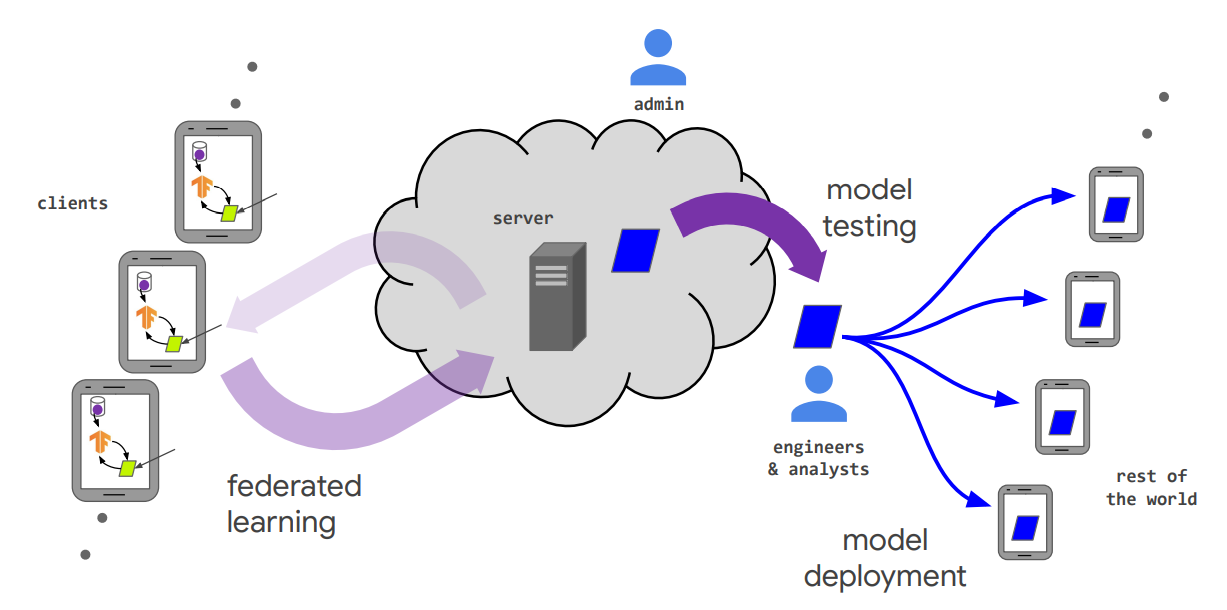
\includegraphics[width=8cm]{assets/structureFL.PNG}
    \caption{The lifecycle of an FL-trained model and the various actors in a federated learning system}
    \label{ Structure FL}
\end{figure}

\subsection{Federated Learning}
Federated learning (FL) is a distributed learning paradigm that aims to train machine learning models from scattered and isolated data. The special features of FL (compared to data center-based distributed training) are : statistical heterogeneity, system constraints and trustworthiness. To provide an answer to these 3 challenges we need to mix knowledge from different fields, including machine learning, wireless communication, mobile computing, distributed systems, and information security. Therefore FL is a truly interdisciplinary research field.  FL has been studied well over the last years and is still developping. However, the traditional FL framework still faces some problems which reduce the reliability of the whole system. These problems detailed in \cite{wang_blockchain-based_2021} are the following : single point of failure, false data and the lalck of incentives. \newline \newline - Single point of failure: this problem is based on the fiability of the aggregator which is the central server in a FL system. The structure of FL is presented Figure \ref{fig:TopologyFL}. This aggregator is employed to perform the integration of local training results and to update the global model.  But, if the centralized aggregator is compromised, the whole FL system will go down. The reasons for a compromised aggregator are : an intentionally dishonest aggregation, an accidental network connection failure, or even an unexpected external attack. \newline \newline -False data: despite the predefined protocols, and due to the huge number of clients in a FL mmodel we have to assume that not all the clients are honest and will use the model as expected. As a consequence, it may exist rogue clients who submit false data about their local training results. Therefore, the global performance of the model can be strongly affected. Besides, the whole FL system might be attacked by malicious clients via other means, such as training the local models using partial datasets. \newline \newline -The lack of incentive methods:  The lack of incentives: in most of the traditional FL, clients contribute their computing powers without receiving any payments, this lead to the difficulty of encouraging clients to follow rigorously the protocol. Therefore the model will lack of reliable data. Moreover, the FL model will also lack of clients. Indeed, as FL requires multiple devices to work collaboratively, especially for the data-intensive training tasks where it needs a large number of participants.
\begin{figure}[!ht]
    \centering
    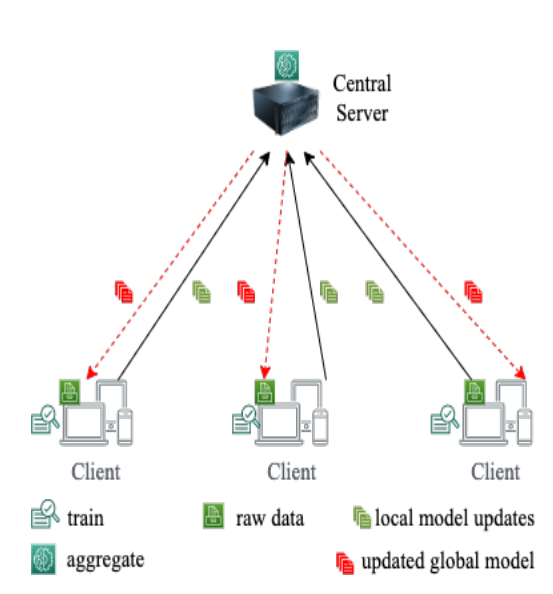
\includegraphics[width=8cm]{assets/topologyFL.PNG}
    \caption{Topology of traditional FL}
    \label{fig:TopologyFL}
\end{figure}

\subsection{Blockchain}
Blockchain, is an emerging technology that come with several attractive properties : decentralization, anonymity, and traceability. These properties has already shown their utilities in different fields. More recently, blockchain begin to be used to address the challenges faced by the acual FL. First, decentralization can be achieved by the deployment of blockchain in FL by replacing the central aggregator by the peer-to-peer blockchain system. On the other hand,  the job of aggregating the global model can be handled by blockchain nodes to avoid the unreliability of the whole FL system usually caused by the centralized server's failure.. Figure \ref{fig:TopologyBC} indicates the topology of block hain. Moreover, blockchain gives verification mechanisms to FL in the name of transaction verification. These mechanisms allows FL model to remove the unqualified or even malicious local model updates before the global model update. Furthermore, blockchain can sucessffully distribute rewards to FL clients to reward their participation and honest behaviors.
\begin{figure}[!ht]
    \centering
    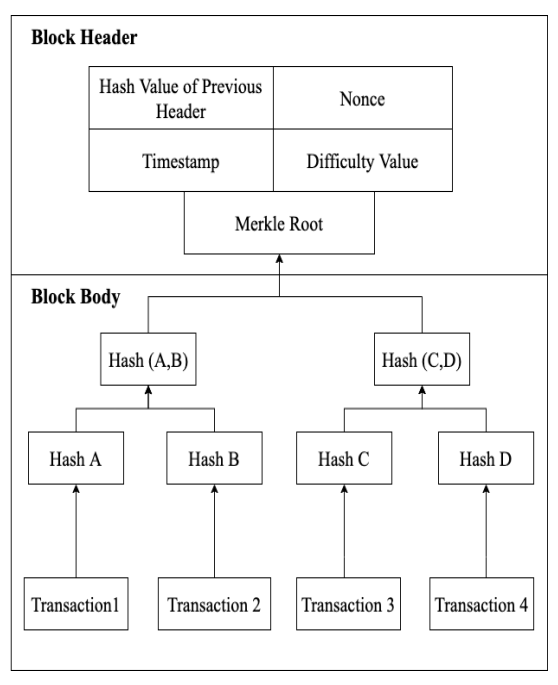
\includegraphics[width=8cm]{assets/topologyBC.PNG}
    \caption{Structure of Block}
    \label{fig:TopologyBC}
\end{figure}

\subsection{Crowdsourcing}

To be done

\section{Motivation}

In the present time, the use of Machine learning (ML) is constantly increasing in every field. Thus, lots of data are generated and gathered from massive end users to train ML models which bring benefits in terms improve the serices offered to people. Therefore, ML framework usually requires end devices to transfer the collected data to the central server for training. But, this process causes two challenges : A large amount of communication resources is requirred to transfer data. Then, the submission of raw data increases the risk of privacy leakage, which making data owners unwilling to upload data to the central server by fear of security. FL paired with blockchain appeared to be a good solution to solve this problem as well as the actual limits of FL mentionned earlier (single point of failure, false data and the lalck of incentives).

\subsection{Crowdsourcing issues}

To be done

\section{Blockchain-based Federated Learning}

Although Federated Learning allows for participants to contribute their local data without it being revealed, it faces issues in data security and in accurately paying participants for quality data contributions. Many researches have already been published in this fiels : 
\newline \newline \cite{martinez_record_2019} propose an EOS Blockchain design and workflow to establish data security, a novel validation error based metric upon which \cite{martinez_record_2019} qualify gradient uploads for payment, and implement a small example of the blockchain Federated Learning model to analyze its performance. This workflow is designed for scalable recording and rewarding of gradients using both blockchain and off-chain databases of records at the same time. Their implementation on a small set of clients demonstrate that the blockchain does not interfere with the federated learning aggregation, while limiting the number of uploads and validating the claimed data cost per device. 
\newline \newline \cite{awan_poster_2019} propose a blockchain-based privacy-preserving federated learning (BC-based PPFL) framework, which leverages the immutability and decentralized trust properties of blockchain to provide provenance of model updates. This framework is based on gradient aggregation over private data following a cryptographic protocol.
\newline \newline \cite{korkmaz_chainfl_2020} propose a decentralized federated learning approach named Chain FL that makes use of the blockchain to delegate the responsibility of storing the model to the nodes on the network instead of a centralized server. This methods doesn’t effect results compared to traditional federated learning as they use the update steps the same way. However, results are slightly worse compared to classical machine learning.
\newline \newline \cite{sharma_2020} propose a distributed computing defence framework for sustainable society using the features of blockchain technology and federated learning. This framework provides security against misbehavior detection in lightweight Internet of Medical Things (IoMT) devices, particularly in the artificial pancreas system (APS). The proposed approach employs privacy-preserving bidirectional long-short term memory (BiLSTM) and augments the security through the integration of Blockchain technology based on Ethereum smart contract environment.
\newline \newline In the work \cite{li_crowdsfl_2020} propose a crowdsourcing framework named CrowdSFL, that users can implement crowdsourcing with less overhead and higher security. Besides, to protect the privacy of participants, this framework include a new re-encryption algorithm based on Elgamal to ensure that interactive values and other information will not be exposed to other participants outside the workflow. As a result, this method is proved to be superior to some similar work in accuracy, efficiency, and overhead.
\newline \newline This paper \cite{chen_2020} proposes a federated learning architecture based on the alliance chain, which defines a complete life cycle for the federated learning process based on blockchain technology. By combining it with the aggregation algorithm of federated learning, and by using knowledge distillation technology to extract network knowledge, the model compressed data before entering the block network for propagation, which reduces the load on the entire blockchain network while providing a better protection for data.
\newline \newline \cite{kumar_2021} propose a framework that collects a small amount of data from different sources (various hospitals) and trains a global deep learning model using blockchain based federated learning. Additionally they collect real-life COVID-19 patients data, which is, open to the research community. The security of local parameters, the learning quality, and the varying computing and communication resources, are crucial issues that remain unexplored in federated learning schemes. 
\newline \newline \cite{guo_2020} propose a data sharing mechanism that combines blockchain and federated learning over smart city. The security of local parameters, the learning quality, and the varying computing and communication resources, are crucial issues that remain unexplored in federated learning schemes. In response to the shortcomings of the original method, this paper designed the work nodes selection algorithm to enhance effectiveness of the federated learning task, and designed a consensus incentivemechanism to encourage the work node to more actively participate in the task. Combining this method with differential privacy technology is a good balance between privacy security and the practicality of the model
\newline \newline \cite{lu_2021} propose a general privacy-preserving federated learning scheme, which integrates blockchain with federated learning, for beyond 5G networks. Furthermore, this paper introduce potential application scenarios of the proposed scheme in beyond 5G. In the proposed scheme, the blockchain is used to maintain learning parameters and verify their accuracies, which can enhance the learning security and quality.
\newline \newline \cite{ma_2021} propose a blockchain-based federated learning framework and a protocol to transparently evaluate each participant's contribution. The framework protects all parties' privacy in the model building phase and transparently evaluates contributions based on the model updates. Collaborative model development and privacy protection are critical considerations while training a global deep learning model. This method was tested on the handwriting digits dataset and demonstrate successful contributions evaluation.
\newline \newline To overcome computational complexity and privacy problems, \cite{durga_fled_2022} proposes the blockchain empowered federated framework to enhance the perception of multiple sources of heterogeneous CT images. It is based on sharing the data among the hospitals while maintaining privacy and security. Also, an ensemble of capsule networks and extreme learning machines are used for effective feature extraction and classification to detect the COVID-19 among the different sources of publicly available heterogenous CT image datasets. Besides, federated learning is adopted for the collaborative training of hospitals backed with blockchain technology. In addition, the combination of chaotic encryption keys in the process of data retrieval and sharing process has added more trust in terms of maintaining privacy and security. 
\newline \newline In the work \cite{lu_2020}, the problem of edge data sharing among vehicles in an internet of vehicles (IoV) framework is studied. This work proposes a hybrid blockchain mechanism that includes the permissioned blockchain and the local directed acyclic graph in IoV. Based on the hybrid blockchain mechanism, it proposed the asynchronous federated learning scheme and further improved the learning efficiency by using DRL to select the optimized participating nodes. By integrating learning parameters into the blockchain, the qualities of learned models can be then be verified through the two-stage verification.
\newline \newline \cite{lee_2021}, gaves a short overview of blockchain and federated learning and showed how blockchain technology can enhance and solve privacy issues. Moreover, it presents an application of a blockchain federated learning framework in the industrial, vehicle network, and healthcare sectors.

\subsection{Impact on machine learning}

\subsubsection{Training}
%What is the impact of blockchain on the training of machine learning models?
Blockchain can be used to train machine learning models in a privacy-compliant way \cite{ladia_2019}), using a decentralized advanced-Proof-of-Work (aPoW) algorithm \cite{kusi_2020}, and that blockchain can be used to solve issues with traditional machine learning models, such as the lack of data privacy and the need for continuous training \cite{ding_2022}. \cite{xu_2022} suggests that blockchain-based crowdsourcing can be used to collect and annotate data for machine learning models.

\subsubsection{Sharing}
%What is the impact of blockchain on the sharing of machine learning models?
Blockchain can also be used to share machine learning models while preserving privacy. \cite{ladia_2019}), \cite{lu_2020}, and \cite{lee_2021} all suggest that blockchain can be used for this purpose. \cite{kurtulmus_2018} suggests that blockchain can be used to facilitate the exchange of machine learning models. It is suggested that blockchain can be used to share machine learning models while preserving privacy.

\section{Research lines}

\subsection{Security issues: privacy}

There are many security problems neglected in federated learning, Indeed, FL allows for participants to contribute their local data to a common goal, thus, it faces issues in data security. To answer this challenge, FL provides an attractive structure (presented in \cite{kairouz_advances_2021}) for decomposing the overall machine learning workflow into the approachable modular units we desire. One of the primary attractions of the federated learning model is that it can provide a level of privacy to participating users through data minimization: the raw user data never leaves the device, and only updates to models (e.g., gradient updates) are sent to the central server. These model updates are more focused on the learning task at hand than is the raw data (i.e. they contain strictly no additional information about the user, and typically significantly less, compared to the raw data), and the individual updates only need to be held ephemerally by the server. To solve this accuracy problem, \cite{weng_2019} present a distributed, secure, and fair deep learning framework. \cite{nguyen_2020} provide a state-of-art survey on the integration of blockchain with 5G networks and beyond. \cite{kumar_2020} introduce a secure and decentralized training for distributed data. \cite{zhang_2020} propose a new architecture based on federated learning to relieve transmission load and address privacy concerns of providers. \cite{otoum_2020} introduce a solution that integrates both federated learning and blockchain to ensure both data privacy and network security. The security of federated learning is increasingly being questioned, due to the malicious clients or central servers' constant attack to the global model or user privacy data. To address these security issues \cite{li_2021} propose a decentralized federated learning framework based on blockchain, i.e., a Blockchain-based Federated Learning framework with Committee consensus (BFLC). \cite{liu_2020} propose a blockchain-based secure FL framework to create smart contracts and prevent malicious or unreliable participants from involving in FL. \cite{9170905} introduce the digital twin wireless networks (DTWN) by incorporating digital twins into wireless networks, to migrate real-time data processing and computation to the edge plane. In further \cite{xu_bafl_2021} propose the concept of device's score and use entropy weight method to measure the quality of model update. Other influential work includes \cite{lu_2020}.

\subsubsection{Impact on security and privacy}
%What is the impact of blockchain on the security of machine learning models?
Blockchain can be used to improve the security of machine learning models. \cite{chen_2020} found that the blockchain technique can be used to design a decentralized privacy-preserving and secure machine learning system. \cite{fadaeddini_2019} found that the proposed framework uses the Stellar Blockchain infrastructure for secure decentralized training of the deep models. \cite{goel_2019} found that the proposed approach provides security to both deep learning model and the biometric template. \cite{wang_ai_2020} found that the proposed system obtains comparable performance with that of conventional distributed systems, and bounded performance in the case of Byzantine attacks. Therefore, blockchain appears to be a promising solution for improving the security of machine learning models.\newline
%What is the impact of blockchain on the privacy of machine learning models?
Blockchain also can be used to train machine learning models while preserving privacy. \cite{ladia_2019}, \cite{kim_2019}, \cite{chen_2018}, and \cite{weng_2019} all propose different ways to do this. These papers suggest that blockchain is a promising solution for training machine learning models while preserving privacy.

\subsection{Quality management: incentive}

There are many security problems neglected in federated learning, for example, the participants may behave incorrectly in gradient collecting or parameter updating, and the server may be malicious as well. In FL processing, the data quality shared by usersdirectly affects the accuracy of the federated learning model, and how to encourage more data owners to share data is crucial. Inother words, how to design a good incentive mechanism is the key problem in FL. 
\newline \newline \cite{weng_2019} present a distributed, secure, and fair deep learning framework named \textit{DeepChain} to solve these problems. This technique provides a promising privacy preservation for mobile devices while simultaneously ensuring high learning performance \cite{kang_2019}. \cite{liu_fedcoin_2020} propose FedCoin, a blockchain-based peer-to-peer payment system for FL to enable a feasible SV based profit distribution. \cite{lin_2022} propose a novel Wirelessly Powered Edge intelliGence (WPEG) framework, which aims to achieve a stable, robust, and sustainable edge intelligence by energy harvesting (EH) methods. \cite{wang_2020} propose SFAC, a secure federated learning framework for UAV-assisted MCS. A new ecosystem of ML model trading over a trusted Blockchain-based network is proposed \cite{nguyen_2021}. Problems, however, can arise if there is a lack of quality data for AI-model training, scalability, and maintenance. \cite{chaabene_2022} propose a data-centric federated learning architecture leveraged by a public blockchain and smart contracts to overcome this significant issue. The proposed approach employs privacy-preserving bidirectional long-short term memory (BiLSTM) and augments the security through the integration of Blockchain technology based on Ethereum smart contract environment \cite{rahmadika_2022}. While several works focus on strategic incentive designs and client selection to overcome this problem, there is a major knowledge gap in terms of an overall design tailored to the foreseen digital economy, including Web 3.0, while simultaneously meeting the learning objectives. To address this gap \cite{pandey_2022} propose a contribution-based tokenized incentive scheme, namely \texttt{FedToken}, backed by blockchain technology that ensures fair allocation of tokens amongst the clients that corresponds to the valuation of their data during model training. Other influential work includes \cite{lu_2020}. 
\begin{figure}[!ht]
    \centering
    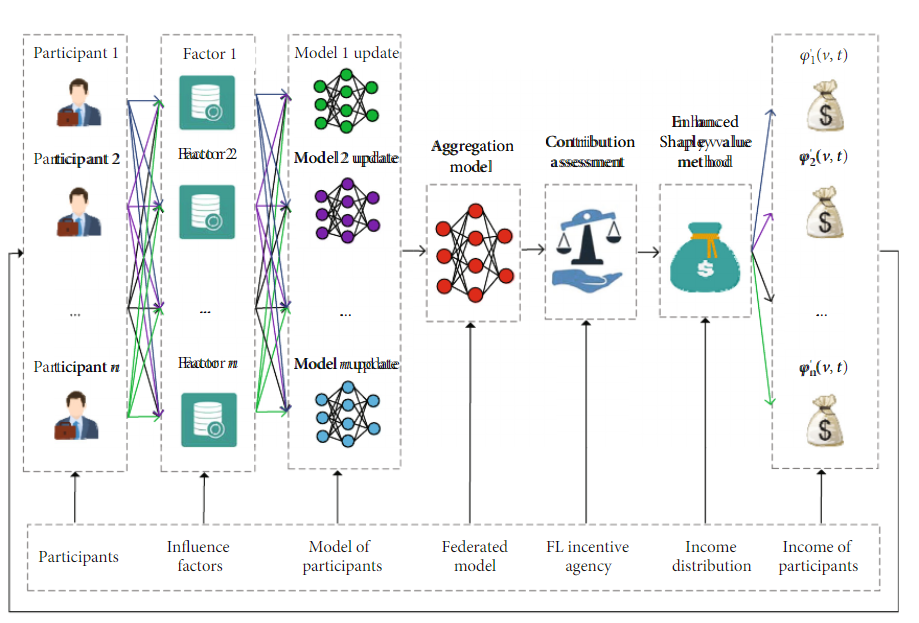
\includegraphics[width=8cm]{assets/incentiveGraph.PNG}
    \caption{FL incentive model}
    \label{fig:incentive_graph}
\end{figure}
\newline \newline In his work, \cite{Weijie_Tan} propose an incentive mechanism based on the enhanced Shapley value method for FL. In this mechanism presented figure \cite{fig:incentive_graph}, the enhanced Shapley value method is proposed to measure income distribution, which takes multiple influence factors as weights. The analytic hierarchy process (AHP) is used to find the corresponding weight value of the influence factors. Finally, the numerical experiments are carried to verify the performance of the proposed incentive mechanism. 

\subsubsection{Impact on incentive models}
%What is the impact of blockchain on incentive models of federated learning?
Blockchain can be used to incentivize federated learning. \cite{kumar_2020}, \cite{pandey_2022}, \cite{wang_2022} and \cite{martinez_record_2019} all found that blockchain can be used to create a value-driven incentive mechanism, a contribution-based tokenized incentive scheme, an incentive mechanism to allocate resources, and establish data security and accurately pay participants, respectively. This incentivizes clients to participate in federated learning, which improves the efficiency of the training. Consequently, blockchain does have an impact on incentive models of federated learning.\newline
%How can blockchain be used to create new incentive models for federated learning?
Blockchain also can be used to create new incentive models for federated learning. \cite{kumar_2020} found that blockchain technology can be used to create a value-driven incentive mechanism for federated learning. \cite{wang_2022} found that a two-stage Stackelberg game can be used to allocate resources for clients in blockchain-based federated learning. \cite{goncalves_2022} found that a blockchain-based federated learning framework can be used to increment the system security using an incentive mechanism. Together, these papers suggest that blockchain can be used to create new incentive models for federated learning.


%\section{Research problem}

%\section{Related work}

%\section{Planned solution}

%\section{Task assignment and goal}


%\section{Electronic Submission}
%\label{submission}
%
%Submission to MLSys 2023 will be entirely electronic, via a web site
%(not email). Information about the submission process and \LaTeX\ templates
%are available on the conference web site at:
%\begin{center}
%\textbf{\texttt{https://www.mlsys.org/}}
%\end{center}
%
%The guidelines below will be enforced for initial submissions and
%camera-ready copies. Here is a brief summary:
%\begin{itemize}
%\item Submissions must be in PDF\@.
%\item The maximum paper length is \textbf{10 pages} excluding references and appendices.
%    (pages 11 and on must contain only references).
%\item \textbf{Do not include author information or acknowledgements} in your
%    initial submission.
%\item Your paper should be in \textbf{10 point Times font}.
%\item Make sure your PDF file only uses Type-1 fonts.
%\item Place figure captions \emph{under} the figure (and omit titles from inside
%    the graphic file itself). Place table captions \emph{over} the table.
%\item References must include page numbers whenever possible and be as complete
%    as possible. Place multiple citations in chronological order.
%\item Do not alter the style template; in particular, do not compress the paper
%    format by reducing the vertical spaces.
%\item Keep your abstract brief and self-contained, one paragraph and roughly
%    4--6 sentences. Gross violations will require correction at the
%    camera-ready phase. The title should have content words capitalized.
%\item Submissions that significantly diverge from the specified format 
%    will be rejected without review.
%\end{itemize}
%
%\subsection{Submitting Papers}
%
%\textbf{Paper Deadline:} The deadline for paper submission that is
%advertised on the conference website is strict. If your full,
%anonymized, submission does not reach us on time, it will not be
%considered for publication. There is no separate abstract submission.
%
%\textbf{Anonymous Submission:} MLSys uses double-blind review: no identifying
%author information may appear on the title page or in the paper
%itself. Section~\ref{author info} gives further details.
%
%\textbf{Simultaneous Submission:} MLSys will not accept any paper which,
%at the time of submission, is under review for another conference or
%has already been published. This policy also applies to papers that
%overlap substantially in technical content with conference papers
%under review or previously published. MLSys submissions must not be
%submitted to other conferences during MLSys's review period. Authors
%may submit to MLSys substantially different versions of journal papers
%that are currently under review by the journal, but not yet accepted
%at the time of submission. Informal publications, such as technical
%reports or papers in workshop proceedings which do not appear in
%print, do not fall under these restrictions.
%
%\medskip
%
%Authors must provide their manuscripts in \textbf{PDF} format.
%Furthermore, please make sure that files contain only embedded Type-1 fonts
%(e.g.,~using the program \texttt{pdffonts} in linux or using
%File/DocumentProperties/Fonts in Acrobat). Other fonts (like Type-3)
%might come from graphics files imported into the document.
%
%Authors using \textbf{Word} must convert their document to PDF\@. Most
%of the latest versions of Word have the facility to do this
%automatically. Submissions will not be accepted in Word format or any
%format other than PDF\@.
%
%Those who use \textbf{\LaTeX} should avoid including Type-3 fonts.
%Those using \texttt{latex} and \texttt{dvips} may need the following
%two commands:
%
%{\footnotesize
%\begin{verbatim}
%dvips -Ppdf -tletter -G0 -o paper.ps paper.dvi
%ps2pdf paper.ps
%\end{verbatim}}
%It is a zero following the ``-G'', which tells dvips to use
%the config.pdf file. Newer \TeX\ distributions don't always need this
%option.
%
%Using \texttt{pdflatex} rather than \texttt{latex}, often gives better
%results. This program avoids the Type-3 font problem, and supports more
%advanced features in the \texttt{microtype} package.
%
%\textbf{Graphics files} should be a reasonable size, and included from
%an appropriate format. Use vector formats (.eps/.pdf) for plots,
%lossless bitmap formats (.png) for raster graphics with sharp lines, and
%jpeg for photo-like images.
%
%The style file uses the \texttt{hyperref} package to make clickable
%links in documents. If this causes problems for you, add
%\texttt{nohyperref} as one of the options to the \texttt{mlsys2023}
%usepackage statement.
%
%
%\subsection{Submitting Final Camera-Ready Copy}
%
%The final versions of papers accepted for publication should follow the
%same format and naming convention as initial submissions, except that
%author information (names and affiliations) should be given. See
%Section~\ref{final author} for formatting instructions.
%
%The footnote, ``Preliminary work. Under review by the MLSys. Do not distribute.'' 
%must be modified to ``\textit{Proceedings of the
%$\mathit{5}^{th}$ MLSys Conference},
%Santa Clara, CA, USA, 2022.
%Copyright 2022 by the author(s).''
%
%For those using the \textbf{\LaTeX} style file, this change (and others) is
%handled automatically by simply changing
%$\mathtt{\backslash usepackage\{mlsys2023\}}$ to
%$$\mathtt{\backslash usepackage[accepted]\{mlsys2023\}}$$
%Authors using \textbf{Word} must edit the
%footnote on the first page of the document themselves.
%
%Camera-ready copies should have the title of the paper as running head
%on each page except the first one. The running title consists of a
%single line centered above a horizontal rule which is $1$~point thick.
%The running head should be centered, bold and in $9$~point type. The
%rule should be $10$~points above the main text. For those using the
%\textbf{\LaTeX} style file, the original title is automatically set as running
%head using the \texttt{fancyhdr} package which is included in the MLSys
%2022 style file package. In case that the original title exceeds the
%size restrictions, a shorter form can be supplied by using
%
%\verb|\mlsystitlerunning{...}|
%
%just before $\mathtt{\backslash begin\{document\}}$.
%Authors using \textbf{Word} must edit the header of the document themselves.
%
%\section{Format of the Paper}
%
%All submissions must follow the specified format.
%
%\subsection{Length and Dimensions}
%
%Papers must not exceed ten (10) pages, including all figures, tables,
%but excluding acknowledgements, references and appendices.
%Acknowledgements should be limited to grants and people who contributed to the paper.
%Any submission that exceeds
%this page limit, or that diverges significantly from the specified format,
%will be rejected without review.
%
%The text of the paper should be formatted in two columns, with an
%overall width of 6.75~inches, height of 9.0~inches, and 0.25~inches
%between the columns. The left margin should be 0.75~inches and the top
%margin 1.0~inch (2.54~cm). The right and bottom margins will depend on
%whether you print on US letter or A4 paper, but all final versions
%must be produced for US letter size.
%
%The paper body should be set in 10~point type with a vertical spacing
%of 11~points. Please use Times typeface throughout the text.
%
%\subsection{Title}
%
%The paper title should be set in 14~point bold type and centered
%between two horizontal rules that are 1~point thick, with 1.0~inch
%between the top rule and the top edge of the page. Capitalize the
%first letter of content words and put the rest of the title in lower
%case.
%
%\subsection{Author Information for Submission}
%\label{author info}
%
%MLSys uses double-blind review, so author information must not appear. If
%you are using \LaTeX\/ and the \texttt{mlsys2023.sty} file, use
%\verb+\mlsysauthor{...}+ to specify authors and \verb+\mlsysaffiliation{...}+ to specify affiliations. (Read the TeX code used to produce this document for an example usage.) The author information
%will not be printed unless \texttt{accepted} is passed as an argument to the
%style file.
%Submissions that include the author information will not
%be reviewed.
%
%\subsubsection{Self-Citations}
%
%If you are citing published papers for which you are an author, refer
%to yourself in the third person. In particular, do not use phrases
%that reveal your identity (e.g., ``in previous work \cite{langley00}, we
%have shown \ldots'').
%
%Do not anonymize citations in the reference section. The only exception are manuscripts that are
%not yet published (e.g., under submission). If you choose to refer to
%such unpublished manuscripts \cite{anonymous}, anonymized copies have
%to be submitted
%as Supplementary Material via CMT\@. However, keep in mind that an MLSys
%paper should be self contained and should contain sufficient detail
%for the reviewers to evaluate the work. In particular, reviewers are
%not required to look at the Supplementary Material when writing their
%review.
%
%\subsubsection{Camera-Ready Author Information}
%\label{final author}
%
%If a paper is accepted, a final camera-ready copy must be prepared.
%%
%For camera-ready papers, author information should start 0.3~inches below the
%bottom rule surrounding the title. The authors' names should appear in 10~point
%bold type, in a row, separated by white space, and centered. Author names should
%not be broken across lines. Unbolded superscripted numbers, starting 1, should
%be used to refer to affiliations.
%
%Affiliations should be numbered in the order of appearance. A single footnote
%block of text should be used to list all the affiliations.
%
%Each distinct affiliations should be listed once. If an author has multiple
%affiliations, multiple superscripts should be placed after the name, separated
%by thin spaces. If the authors would like to highlight equal contribution by
%multiple first authors, those authors should have an asterisk placed after their
%name in superscript, and the term ``\textsuperscript{*}Equal contribution"
%should be placed in the footnote block ahead of the list of affiliations. A
%list of corresponding authors and their emails (in the format Full Name
%\textless{}email@domain.com\textgreater{}) can follow the list of affiliations.
%Ideally only one or two names should be listed.
%
%A sample file with author names is included in the mlsys2023 style file
%package. Turn on the \texttt{[accepted]} option to the stylefile to
%see the names rendered. All of the guidelines above are implemented
%by the \LaTeX\ style file.
%
%\subsection{Abstract}
%
%The paper abstract should begin in the left column, 0.4~inches below the final
%address. The heading `Abstract' should be centered, bold, and in 11~point type.
%The abstract body should use 10~point type, with a vertical spacing of
%11~points, and should be indented 0.25~inches more than normal on left-hand and
%right-hand margins. Insert 0.4~inches of blank space after the body. Keep your
%abstract brief and self-contained, limiting it to one paragraph and roughly 4--6
%sentences. Gross violations will require correction at the camera-ready phase.
%
%\subsection{Partitioning the Text}
%
%You should organize your paper into sections and paragraphs to help
%readers place a structure on the material and understand its
%contributions.
%
%\subsubsection{Sections and Subsections}
%
%Section headings should be numbered, flush left, and set in 11~pt bold
%type with the content words capitalized. Leave 0.25~inches of space
%before the heading and 0.15~inches after the heading.
%
%Similarly, subsection headings should be numbered, flush left, and set
%in 10~pt bold type with the content words capitalized. Leave
%0.2~inches of space before the heading and 0.13~inches afterward.
%
%Finally, subsubsection headings should be numbered, flush left, and
%set in 10~pt small caps with the content words capitalized. Leave
%0.18~inches of space before the heading and 0.1~inches after the
%heading.
%
%Please use no more than three levels of headings.
%
%\subsubsection{Paragraphs and Footnotes}
%
%Within each section or subsection, you should further partition the
%paper into paragraphs. Do not indent the first line of a given
%paragraph, but insert a blank line between succeeding ones.
%
%You can use footnotes\footnote{Footnotes
%should be complete sentences.} to provide readers with additional
%information about a topic without interrupting the flow of the paper.
%Indicate footnotes with a number in the text where the point is most
%relevant. Place the footnote in 9~point type at the bottom of the
%column in which it appears. Precede the first footnote in a column
%with a horizontal rule of 0.8~inches.\footnote{Multiple footnotes can
%appear in each column, in the same order as they appear in the text,
%but spread them across columns and pages if possible.}
%
%\subsection{Figures}
%
%You may want to include figures in the paper to illustrate
%your approach and results. Such artwork should be centered,
%legible, and separated from the text. Lines should be dark and at
%least 0.5~points thick for purposes of reproduction, and text should
%not appear on a gray background.
%
%Label all distinct components of each figure. If the figure takes the
%form of a graph, then give a name for each axis and include a legend
%that briefly describes each curve. Do not include a title inside the
%figure; instead, the caption should serve this function.
%
%Number figures sequentially, placing the figure number and caption
%\emph{after} the graphics, with at least 0.1~inches of space before
%the caption and 0.1~inches after it. The figure caption should be set in
%9~point type and centered unless it runs two or more lines, in which
%case it should be flush left. You may float figures to the top or
%bottom of a column, and you may set wide figures across both columns
%(use the environment \texttt{figure*} in \LaTeX). Always place
%two-column figures at the top or bottom of the page.
%
%\subsection{Algorithms}
%
%If you are using \LaTeX, please use the ``algorithm'' and ``algorithmic''
%environments to format pseudocode. These require
%the corresponding stylefiles, algorithm.sty and
%algorithmic.sty, which are supplied with this package.
%Algorithm~\ref{alg:example} shows an example.
%
%\begin{algorithm}[tb]
%   \caption{Bubble Sort}
%   \label{alg:example}
%\begin{algorithmic}
%   \STATE {\bfseries Input:} data $x_i$, size $m$
%   \REPEAT
%   \STATE Initialize $noChange = true$.
%   \FOR{$i=1$ {\bfseries to} $m-1$}
%   \IF{$x_i > x_{i+1}$}
%   \STATE Swap $x_i$ and $x_{i+1}$
%   \STATE $noChange = false$
%   \ENDIF
%   \ENDFOR
%   \UNTIL{$noChange$ is $true$}
%\end{algorithmic}
%\end{algorithm}
%
%\subsection{Tables}
%
%You may also want to include tables that summarize material. Like
%figures, these should be centered, legible, and numbered consecutively.
%However, place the title \emph{above} the table with at least
%0.1~inches of space before the title and the same after it, as in
%Table~\ref{sample-table}. The table title should be set in 9~point
%type and centered unless it runs two or more lines, in which case it
%should be flush left.
%
%% Note use of \abovespace and \belowspace to get reasonable spacing
%% above and below tabular lines.
%
%\begin{table}[t]
%\caption{Classification accuracies for naive Bayes and flexible
%Bayes on various data sets.}
%\label{sample-table}
%\vskip 0.15in
%\begin{center}
%\begin{small}
%\begin{sc}
%\begin{tabular}{lcccr}
%\toprule
%Data set & Naive & Flexible & Better? \\
%\midrule
%Breast    & 95.9$\pm$ 0.2& 96.7$\pm$ 0.2& $\surd$ \\
%Cleveland & 83.3$\pm$ 0.6& 80.0$\pm$ 0.6& $\times$\\
%Glass2    & 61.9$\pm$ 1.4& 83.8$\pm$ 0.7& $\surd$ \\
%Credit    & 74.8$\pm$ 0.5& 78.3$\pm$ 0.6&         \\
%Horse     & 73.3$\pm$ 0.9& 69.7$\pm$ 1.0& $\times$\\
%Meta      & 67.1$\pm$ 0.6& 76.5$\pm$ 0.5& $\surd$ \\
%Pima      & 75.1$\pm$ 0.6& 73.9$\pm$ 0.5&         \\
%Vehicle   & 44.9$\pm$ 0.6& 61.5$\pm$ 0.4& $\surd$ \\
%\bottomrule
%\end{tabular}
%\end{sc}
%\end{small}
%\end{center}
%\vskip -0.1in
%\end{table}
%
%Tables contain textual material, whereas figures contain graphical material.
%Specify the contents of each row and column in the table's topmost
%row. Again, you may float tables to a column's top or bottom, and set
%wide tables across both columns. Place two-column tables at the
%top or bottom of the page.
%
%\subsection{Citations and References}
%
%Please use APA reference format regardless of your formatter
%or word processor. If you rely on the \LaTeX\/ bibliographic
%facility, use \texttt{natbib.sty} and \texttt{mlsys2023.bst}
%included in the style-file package to obtain this format.
%
%Citations within the text should include the authors' last names and
%year. If the authors' names are included in the sentence, place only
%the year in parentheses, for example when referencing Arthur Samuel's
%pioneering work \yrcite{Samuel59}. Otherwise place the entire
%reference in parentheses with the authors and year separated by a
%comma \cite{Samuel59}. List multiple references separated by
%semicolons \cite{kearns89,Samuel59,mitchell80}. Use the `et~al.'
%construct only for citations with three or more authors or after
%listing all authors to a publication in an earlier reference \cite{MachineLearningI}.
%
%Authors should cite their own work in the third person
%in the initial version of their paper submitted for blind review.
%Please refer to Section~\ref{author info} for detailed instructions on how to
%cite your own papers.
%
%Use an unnumbered first-level section heading for the references, and use a
%hanging indent style, with the first line of the reference flush against the
%left margin and subsequent lines indented by 10 points. The references at the
%end of this document give examples for journal articles \cite{Samuel59},
%conference publications \cite{langley00}, book chapters \cite{Newell81}, books
%\cite{DudaHart2nd}, edited volumes \cite{MachineLearningI}, technical reports
%\cite{mitchell80}, and dissertations \cite{kearns89}.
%
%Alphabetize references by the surnames of the first authors, with
%single author entries preceding multiple author entries. Order
%references for the same authors by year of publication, with the
%earliest first. Make sure that each reference includes all relevant
%information (e.g., page numbers).
%
%Please put some effort into making references complete, presentable, and
%consistent. If using bibtex, please protect capital letters of names and
%abbreviations in titles, for example, use \{B\}ayesian or \{L\}ipschitz
%in your .bib file.
%
%\subsection{Software and Data}
%
%We strongly encourage the publication of software and data with the
%camera-ready version of the paper whenever appropriate. This can be
%done by including a URL in the camera-ready copy. However, do not
%include URLs that reveal your institution or identity in your
%submission for review. Instead, provide an anonymous URL or upload
%the material as ``Supplementary Material'' into the CMT reviewing
%system. Note that reviewers are not required to look at this material
%when writing their review.

%\section{Conclusion}
%
%% Acknowledgements should only appear in the accepted version.
%\section*{Acknowledgements}
%
%\textbf{Do not} include acknowledgements in the initial version of
%the paper submitted for blind review.
%
%If a paper is accepted, the final camera-ready version can (and
%probably should) include acknowledgements. In this case, please
%place such acknowledgements in an unnumbered section at the
%end of the paper. Typically, this will include thanks to reviewers
%who gave useful comments, to colleagues who contributed to the ideas,
%and to funding agencies and corporate sponsors that provided financial
%support.


% In the unusual situation where you want a paper to appear in the
% references without citing it in the main text, use \nocite
\nocite{langley00}

\bibliography{biblatex}
\bibliographystyle{mlsys2023}


%%%%%%%%%%%%%%%%%%%%%%%%%%%%%%%%%%%%%%%%%%%%%%%%%%%%%%%%%%%%%%%%%%%%%%%%%%%%%%%
%%%%%%%%%%%%%%%%%%%%%%%%%%%%%%%%%%%%%%%%%%%%%%%%%%%%%%%%%%%%%%%%%%%%%%%%%%%%%%%
% SUPPLEMENTAL CONTENT AS APPENDIX AFTER REFERENCES
%%%%%%%%%%%%%%%%%%%%%%%%%%%%%%%%%%%%%%%%%%%%%%%%%%%%%%%%%%%%%%%%%%%%%%%%%%%%%%%
%%%%%%%%%%%%%%%%%%%%%%%%%%%%%%%%%%%%%%%%%%%%%%%%%%%%%%%%%%%%%%%%%%%%%%%%%%%%%%%

%\appendix
%\section{Please add supplemental material as appendix here}
%
%Put anything that you might normally include after the references as an appendix here, {\it not in a separate supplementary file}. Upload your final camera-ready as a single pdf, including all appendices.

%%%%%%%%%%%%%%%%%%%%%%%%%%%%%%%%%%%%%%%%%%%%%%%%%%%%%%%%%%%%%%%%%%%%%%%%%%%%%%%
%%%%%%%%%%%%%%%%%%%%%%%%%%%%%%%%%%%%%%%%%%%%%%%%%%%%%%%%%%%%%%%%%%%%%%%%%%%%%%%


\end{document}


% This document was modified from the file originally made available by
% Pat Langley and Andrea Danyluk for ICML-2K. This version was created
% by Iain Murray in 2018. It was modified from a version from Dan Roy in
% 2017, which was based on a version from Lise Getoor and Tobias
% Scheffer, which was slightly modified from the 2010 version by
% Thorsten Joachims & Johannes Fuernkranz, slightly modified from the
% 2009 version by Kiri Wagstaff and Sam Roweis's 2008 version, which is
% slightly modified from Prasad Tadepalli's 2007 version which is a
% lightly changed version of the previous year's version by Andrew
% Moore, which was in turn edited from those of Kristian Kersting and
% Codrina Lauth. Alex Smola contributed to the algorithmic style files.
